\documentclass{article}
\usepackage{polski}
\usepackage{graphicx}
\usepackage[a4paper, total={6in, 10in}]{geometry}

\title{System Zarządzania Magazynami - dokumentacja}
\author{Krzysztof Czerwiński}
\date{Bazy Danych 2, Maj 2024r.}

\begin{document}

\maketitle

\section{Opis problemu i funkcjonalności}
Prosta biblioteka ma realizować funkcję systemu zarządzania produktami w wielu bazach danych. System uwzględnia istnienie jednej centralnej bazy danych, która zawiera informacje o produktach, oraz ich sumaryczną ilość z wszystkich magazynów. Bazy danych poszczególnych produktów zawierają informacje tylko o kodach produktów i ich ilości w danym magazynie. Centralna baza danych umożliwia składanie zamówień w poszczególnych magazynach i aktualizowania ilości produktów w nich przechowywanych. Stworzone zostały odpowiednie wyzwalacze i procedury, aby system wilu baz danych był spójny.
\section{Opis typów danych oraz metod udostępnionych w ramach API}
Do obsługi API stworzony został prosty interfejs graficzny, korzysta on z następującego API:
\begin{itemize}
    \item lista produktów wraz z ich szczegółami
    \item dodanie produktu do koszyka
    \item wyświetlnie koszyka
    \item potwierdzenie zamówienia związane z potwierdzeniem lub odrzuceniem transakcji
    \item zmiana ilości produktów w poszczególnym magazynie
    \item centralne zablokowanie produktu
    \item wyświetlanie listy zamówień
    \item wyświetlanie szczegółów zamówień
\end{itemize}
\subsection{Szczegółowa dokumentacja API}
Aby zobaczyć szczegółową dokumentację endpointów należy użyć brancha \verb|rest|, zbudować i uruchomić projekt oraz otworzyć url \verb|http://localhost:8080/swagger-ui/index.html|. 
\section{Skrypt testujący funkcjonalność API}
API może być testowane przy pomocy Swagger-UI, aby uruchomić Swagger UI postępuj według 2.1. Framework ten stanowi zaróno dokumentacje jak i pozwala wykonywanie przykładowych requestów - czyli testowania API.
\section{Baza danych}
Skrypty zawarte w repoytorium oraz kod zakładają obsługę 1 centralnej bazy danych, i 4 baz dla poszczególnych magazynów. W obecnej implementacji wszystkie bazy danych znajdują się na jednym serwerze, ograniczenie wynika z tworzenia bazy danych przy pomocy Dockera. Tworząc bazy danych ręcznie, na środowisku Windowsowym możemy w prosty sposób postawić każdą bazę danych na osobnym serwerze.
\begin{figure}[h!]
    \centering
    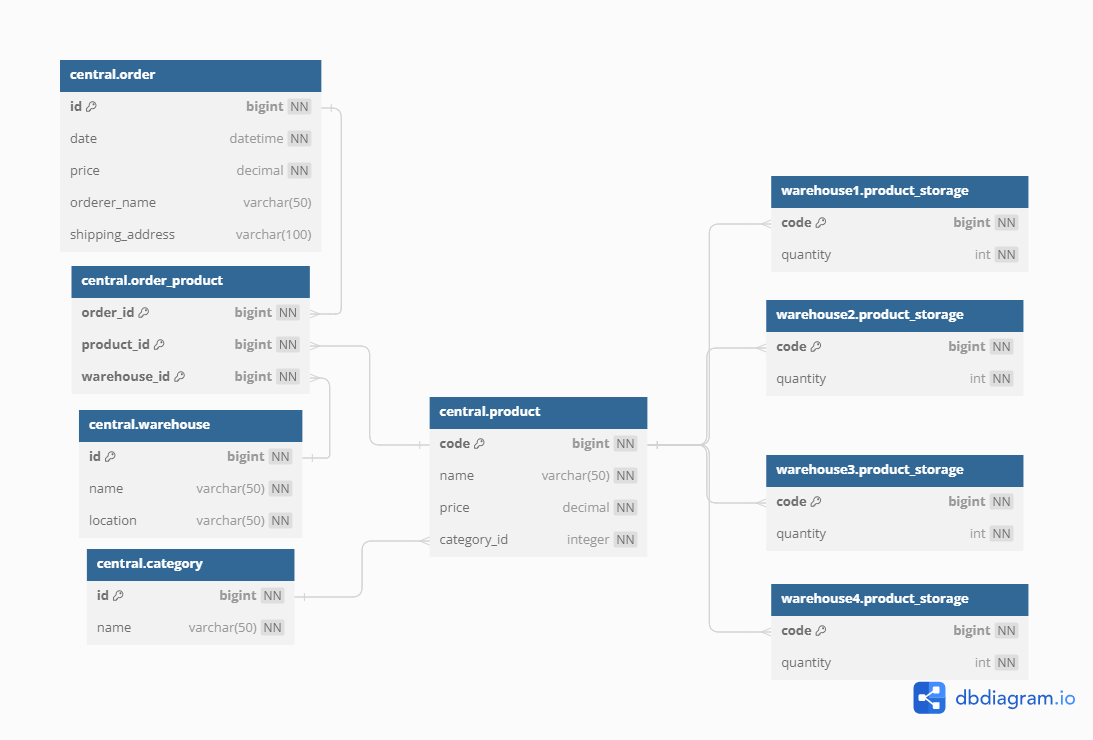
\includegraphics[width = \textwidth]{warehouse-distributed-system.png}
    \caption{Diagram ERD uwzględniający wszystkie 5 baz danych}
    \label{fig:enter-label}
\end{figure}
\newpage
\section{Tworzenie serwera bazy danych}
Aby uruchomić serwer i stworzyć bazy danych z przykładowymi danymi należy upewnić się, że mamy zainstalowane na naszej maszynie oprogramowanie Docker i Docker compose. \\
Należy upewnić się, że uzupełniliśmy szczegóły dotyczące deploymentu w pliku \verb|.env|, należy szczególnie zwrócić uwagę na paremetry dotyczące otwartych portów oraz dotyczących tworzenia baz danych i dodawania do nich danych testowych. \\
Komenda tworząca i uruchamiająca serwer, oraz dodająca przykładowe dane:\\ \verb|docker compose --env-file .env.dev up -d|, gdzie \verb|--env-file| jest opcjonalnym parametrem przekazującym nazwę pliku ze zmiennymi środowiskowymi.

\section{Uruchamianie aplikacji}
Przed uruchomieniem aplikacji należy uzupełnić parametry dotyczące połączenia do bazy danych w pliku \verb|secrets.properties|. Wzór wymaganych parametrów znajduje się w pliku \verb|secrets-dev.properties|. \\
Należy również upewnić się, iż na naszej maszynie jest zainstalowana Java w wersji 21. \\
Po wprowadzeniu szczegółów należy uruchomić plik \verb|.jar| przy pomocy polecenia \verb|java -jar app.jar|.
\newpage
\section{Przykładowa aplikacja}
Aplikacje w trybie developerkim można przetestować korzystając z URL: \verb|http://localhost:8080|.
\begin{figure}[h!]
    \centering
    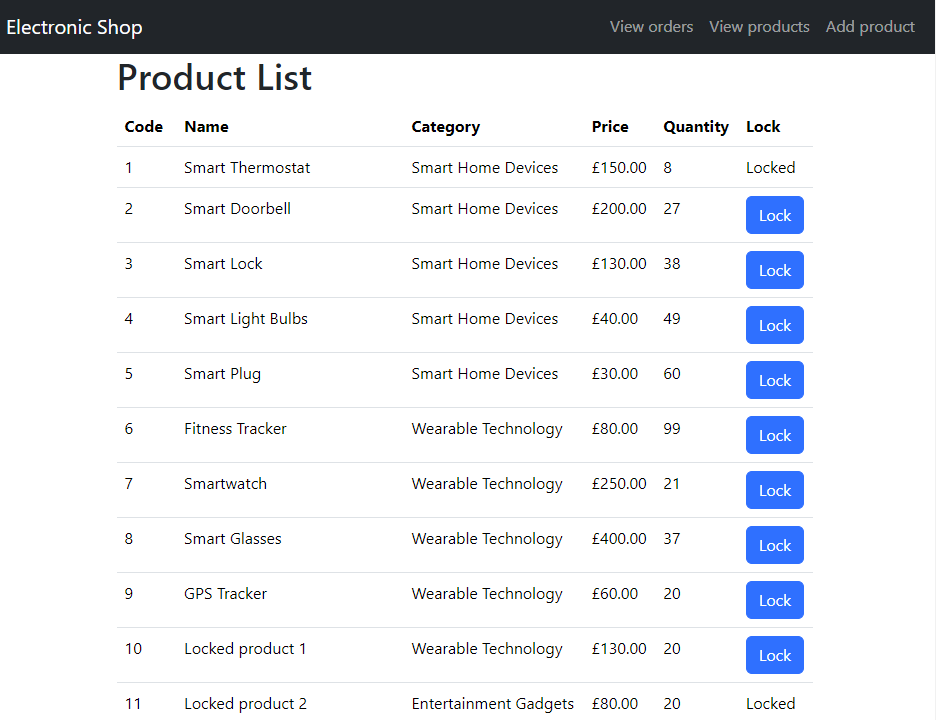
\includegraphics[width = \textwidth]{admin_products_2.png}
    \caption{Przykładowy ekran koszyka aplikacji}
    \label{fig:enter-label}
\end{figure}
\section{Testy jednostkowe}
Dla każdego z endpointów zostały stworzone testy jednostkowe testujące najważniejsze funkcjonalności.
\section{Podsumowanie}
Wszystkie skrypty oraz kody źródłowe bibilioteki oraz aplikacji są załączone w repozytorium. \\
Link do repozytorium: \verb|https://github.com/k-czerwinski/warehouse-distributed-system|
\end{document}
